We perform the analysis on a dataset corresponding to $187\pm7\ipb$ integrated luminosity.

Table~\ref{tab:zzselection_all} shows the number of events observed in 
data, comparing to the expected background contribution at the \zz{} 
preselection level. The background estimation was discussed at Section~\ref{sec:backgrounds}. 
Figure~\ref{fig:zz_0j_1} the distributions of key analysis variables observed in data, comparing 
to the SM expectations from simulation in the 0-jet bin final state.  

%%%%%%%%
\begin{table}[!ht]
\begin{center}
\begin{tabular} {c|c|c|cccc}
\hline
 Jet-Bin & data & all bkg. & peaking-$WZ$/$ZZ$ & $\WW$+$\ttbar+tW$ & $\dyll$ & $\Wjets$ \\
\hline
 0-Jet & X & X & X  & X & X & X\\
 1-Jet & X & X & X  & X & X & X\\
% 2-Jet & X & X & X  & X & X & X \\
\hline
\hline
\end{tabular}
\caption{Expected number of signal and background events from the data-driven methods for an 
  integrated luminosity of $187\pm7\ipb$ after applying the $\ZZ$ selection requirements. 
Both statistical and systematic uncertaities are reported. }
   \label{tab:zzselection_all}
  \end{center}
\end{table}
%%%%%%%%

Table~\ref{tab:yield_0j_zzpresel}-\ref{tab:yield_1j_zzpresel} shows the number of observed events after the $\ZZ$ 
selection, compared to the expected number of signal and background events from the data-driven methods for an 
 integrated luminosity of $187\pm7\ipb$ in the 0 and 1 jet bins. 
The MC expectations includes the lepton efficiencies, trigger 
efficiencies, pileup reweighting, higher order reweighting on the $\hzz$ and $\pt$-dependent 
reweighting on $\ZZ$ and the data/simulation scale factors derived in Section~\ref{sec:backgrounds}.  


%%%%%%%%
\begin{table}[!ht]
\begin{center}
\begin{tabular}{c|cc|c}
\hline
sample    & $\mu\mu$   & ee     & TOTAL\\ \hline 
hzz300   & 0.43 $\pm$ 0.01   & 0.31 $\pm$ 0.00   & 0.74 $\pm$ 0.01 \\ \hline 
hww300   & 0.13 $\pm$ 0.00   & 0.10 $\pm$ 0.00   & 0.22 $\pm$ 0.01 \\ \hline 
wjets   & 0.00 $\pm$ 0.00   & 0.26 $\pm$ 0.12   & 0.26 $\pm$ 0.12 \\ \hline 
qqww   & 2.12 $\pm$ 0.07   & 1.43 $\pm$ 0.06   & 3.55 $\pm$ 0.09 \\ \hline 
ggww   & 0.13 $\pm$ 0.01   & 0.09 $\pm$ 0.01   & 0.22 $\pm$ 0.01 \\ \hline 
wz   & 1.22 $\pm$ 0.05   & 0.72 $\pm$ 0.04   & 1.94 $\pm$ 0.06 \\ \hline 
$\zz$   & 2.49 $\pm$ 0.05   & 1.72 $\pm$ 0.04   & 4.21 $\pm$ 0.06 \\ \hline 
$\ttbar$   & 0.28 $\pm$ 0.12   & 0.08 $\pm$ 0.05   & 0.36 $\pm$ 0.13 \\ \hline 
$\tw$   & 0.12 $\pm$ 0.03   & 0.12 $\pm$ 0.03   & 0.24 $\pm$ 0.04 \\ \hline 
$\dytt$   & 0.00 $\pm$ 0.00   & 0.00 $\pm$ 0.00   & 0.00 $\pm$ 0.00 \\ \hline 
$\dyll$   & 1.28 $\pm$ 0.04   & 1.28 $\pm$ 0.04   & 2.57 $\pm$ 0.05 \\ \hline 
SIGNAL   & 0.43 $\pm$ 0.01   & 0.31 $\pm$ 0.00   & 0.74 $\pm$ 0.01 \\ \hline 
BKGD   & 7.78 $\pm$ 0.16   & 5.79 $\pm$ 0.16   & 13.57 $\pm$ 0.23 \\ \hline 
DATA   & 10.00 $\pm$ 3.16   & 8.00 $\pm$ 2.83   & 18.00 $\pm$ 4.24 \\ \hline 
\end{tabular}
\caption{
Expected number of signal and background events from the data-driven methods for an 
  integrated luminosity of $187\pm7\ipb$ after the {\bf $\ZZ$ pre-selection in the 0-Jet bin}. 
Only statistical uncertainties are reported. The MC expectations includes the lepton efficiencies, 
trigger efficiencies, pileup reweighting, 
higher order reweighting on the $\hzz$ and $\pt$-dependent reweighting on $\ZZ$. The $\ttbar$, 
$\tw$, $\ww$, $\dytt$ and $\wjets$ yields include the data/MC scale factors derived in section~\ref{sec:backgrounds}. }
\label{tab:yield_0j_zzpresel}
\end{center}
%\end{table}
%%%%%%%%
%%%%%%%%
%\begin{table}[!ht]
\begin{center}
\begin{tabular}{c|cc|c}
\hline
sample    & $\mu\mu$   & ee     & TOTAL\\ \hline 
hzz300   & 0.24 $\pm$ 0.00   & 0.17 $\pm$ 0.00   & 0.42 $\pm$ 0.01 \\ \hline 
hww300   & 0.08 $\pm$ 0.00   & 0.05 $\pm$ 0.00   & 0.14 $\pm$ 0.00 \\ \hline 
wjets   & 0.00 $\pm$ 0.00   & 0.00 $\pm$ 0.00   & 0.00 $\pm$ 0.00 \\ \hline 
qqww   & 0.54 $\pm$ 0.03   & 0.37 $\pm$ 0.03   & 0.91 $\pm$ 0.04 \\ \hline 
ggww   & 0.04 $\pm$ 0.00   & 0.02 $\pm$ 0.00   & 0.06 $\pm$ 0.00 \\ \hline 
wz   & 0.64 $\pm$ 0.04   & 0.44 $\pm$ 0.03   & 1.09 $\pm$ 0.05 \\ \hline 
zz   & 0.63 $\pm$ 0.02   & 0.46 $\pm$ 0.02   & 1.09 $\pm$ 0.03 \\ \hline 
ttbar   & 0.41 $\pm$ 0.12   & 0.50 $\pm$ 0.15   & 0.91 $\pm$ 0.19 \\ \hline 
tw   & 0.13 $\pm$ 0.03   & 0.15 $\pm$ 0.03   & 0.27 $\pm$ 0.04 \\ \hline 
zttjets   & 0.00 $\pm$ 0.00   & 0.00 $\pm$ 0.00   & 0.00 $\pm$ 0.00 \\ \hline 
$\dyll$   & 1.31 $\pm$ 0.02   & 1.31 $\pm$ 0.02   & 2.62 $\pm$ 0.02 \\ \hline 
SIGNAL   & 0.24 $\pm$ 0.00   & 0.17 $\pm$ 0.00   & 0.42 $\pm$ 0.01 \\ \hline 
BKGD   & 3.78 $\pm$ 0.14   & 3.31 $\pm$ 0.16   & 7.08 $\pm$ 0.21 \\ \hline 
DATA   & 7.00 $\pm$ 2.65   & 1.00 $\pm$ 1.00   & 8.00 $\pm$ 2.83 \\ \hline 
\end{tabular}
\caption{
Expected number of signal and background events from the data-driven methods for an 
  integrated luminosity of $187\pm7\ipb$ after the {\bf $\ZZ$ pre-selection in the 1-Jet bin}. 
Only statistical uncertainties are reported. The MC expectations includes the lepton efficiencies, 
trigger efficiencies, pileup reweighting, 
higher order reweighting on the $\hzz$ and $\pt$-dependent reweighting on $\ZZ$. The $\ttbar$, 
$\tw$, $\ww$, $\dytt$ and $\wjets$ yields include the data/MC scale factors derived in section~\ref{sec:backgrounds}. }
\label{tab:yield_1j_zzpresel}
\end{center}
\end{table}
%%%%%%%%




%%%%%%%%
\begin{table}[!ht]
\begin{center}
\begin{tabular}{c|cc|c}
\hline
sample    & $\mu\mu$   & ee     & TOTAL\\ \hline 
hzz200   & 0.02 $\pm$ 0.00   & 0.01 $\pm$ 0.00   & 0.03 $\pm$ 0.00 \\ \hline 
hww200   & 0.15 $\pm$ 0.01   & 0.11 $\pm$ 0.01   & 0.26 $\pm$ 0.01 \\ \hline 
wjets   & 0.00 $\pm$ 0.00   & 0.02 $\pm$ 0.02   & 0.02 $\pm$ 0.02 \\ \hline 
qqww   & 0.89 $\pm$ 0.04   & 0.58 $\pm$ 0.03   & 1.47 $\pm$ 0.06 \\ \hline 
ggww   & 0.04 $\pm$ 0.00   & 0.04 $\pm$ 0.00   & 0.08 $\pm$ 0.01 \\ \hline 
$\WZ$   & 0.36 $\pm$ 0.03   & 0.22 $\pm$ 0.02   & 0.58 $\pm$ 0.03 \\ \hline 
$\ZZ$   & 0.53 $\pm$ 0.02   & 0.35 $\pm$ 0.02   & 0.88 $\pm$ 0.03 \\ \hline 
$\ttbar$   & 0.06 $\pm$ 0.05   & 0.00 $\pm$ 0.00   & 0.06 $\pm$ 0.05 \\ \hline 
$\tw$   & 0.05 $\pm$ 0.02   & 0.05 $\pm$ 0.02   & 0.09 $\pm$ 0.03 \\ \hline 
$dytt$   & 0.00 $\pm$ 0.00   & 0.00 $\pm$ 0.00   & 0.00 $\pm$ 0.00 \\ \hline 
gamma   & 0.53 $\pm$ 0.01   & 0.53 $\pm$ 0.01   & 1.06 $\pm$ 0.02 \\ \hline 
SIGNAL   & 0.02 $\pm$ 0.00   & 0.01 $\pm$ 0.00   & 0.03 $\pm$ 0.00 \\ \hline 
BKGD   & 2.61 $\pm$ 0.08   & 1.89 $\pm$ 0.05   & 4.50 $\pm$ 0.10 \\ \hline 
DATA   & 2.00 $\pm$ 1.41   & 2.00 $\pm$ 1.41   & 4.00 $\pm$ 2.00 \\ \hline 
\end{tabular}
\caption{Expected number of signal and background events from the data-driven methods for an 
  integrated luminosity of $187\pm7\ipb$ after applying the $\hzz$ ($m_H = 200\GeVcc$) 
selection requirements in the 0-Jet bin. Only statistical uncertainties are reported. 
The MC expectations includes the lepton efficiencies, trigger efficiencies, pileup reweighting, 
higher order reweighting on the $\hzz$ and $\pt$-dependent reweighting on $\ZZ$. The $\ttbar$, 
$\tw$, $\ww$, $\dytt$ and $\wjets$ yields include the data/MC scale factors derived in section~\ref{sec:backgrounds}. }
\label{tab:yield_0j_hzz200}
\end{center}
%\end{table}
%%%%%%%%
%%%%%%%%
%\begin{table}[!ht]
\begin{center}
\begin{tabular}{c|cc|c}
\hline
sample    & $\mu\mu$   & ee     & TOTAL\\ \hline 
hzz200   & 0.00 $\pm$ 0.00   & 0.00 $\pm$ 0.00   & 0.01 $\pm$ 0.00 \\ \hline 
hww200   & 0.00 $\pm$ 0.00   & 0.00 $\pm$ 0.00   & 0.01 $\pm$ 0.00 \\ \hline 
wjets   & 0.00 $\pm$ 0.00   & 0.00 $\pm$ 0.00   & 0.00 $\pm$ 0.00 \\ \hline 
qqww   & 0.01 $\pm$ 0.00   & 0.01 $\pm$ 0.00   & 0.02 $\pm$ 0.01 \\ \hline 
ggww   & 0.00 $\pm$ 0.00   & 0.00 $\pm$ 0.00   & 0.00 $\pm$ 0.00 \\ \hline 
$\WZ$   & 0.00 $\pm$ 0.00   & 0.00 $\pm$ 0.00   & 0.00 $\pm$ 0.00 \\ \hline 
$\ZZ$   & 0.00 $\pm$ 0.00   & 0.00 $\pm$ 0.00   & 0.01 $\pm$ 0.00 \\ \hline 
$\ttbar$   & 0.01 $\pm$ 0.01   & 0.00 $\pm$ 0.00   & 0.01 $\pm$ 0.01 \\ \hline 
$\tw$   & 0.01 $\pm$ 0.01   & 0.00 $\pm$ 0.00   & 0.01 $\pm$ 0.01 \\ \hline 
$\dytt$   & 0.00 $\pm$ 0.00   & 0.00 $\pm$ 0.00   & 0.00 $\pm$ 0.00 \\ \hline 
$\dyll$   & 0.02 $\pm$ 0.00   & 0.02 $\pm$ 0.00   & 0.04 $\pm$ 0.00 \\ \hline 
SIGNAL   & 0.00 $\pm$ 0.00   & 0.00 $\pm$ 0.00   & 0.01 $\pm$ 0.00 \\ \hline 
BKGD   & 0.06 $\pm$ 0.02   & 0.03 $\pm$ 0.01   & 0.10 $\pm$ 0.02 \\ \hline 
DATA   & 0.00 $\pm$ 0.00   & 0.00 $\pm$ 0.00   & 0.00 $\pm$ 0.00 \\ \hline 
\end{tabular}
\caption{Expected number of signal and background events from the data-driven methods for an 
  integrated luminosity of $187\pm7\ipb$ after applying the {\bf $\hzz$ ($m_H = 200\GeVcc$) selection in the 0-Jet bin}. 
Only statistical uncertainties are reported. 
The MC expectations includes the lepton efficiencies, trigger efficiencies, pileup reweighting, 
higher order reweighting on the $\hzz$ and $\pt$-dependent reweighting on $\ZZ$. The $\ttbar$, 
$\tw$, $\ww$, $\dytt$ and $\wjets$ yields include the data/MC scale factors derived in section~\ref{sec:backgrounds}. }
\label{tab:yield_1j_hzz200}
\end{center}
\end{table}
%%%%%%%%



%%%%%%%%
\begin{table}[!ht]
\begin{center}
\begin{tabular}{c|cc|c}
\hline
sample    & $\mu\mu$   & ee     & TOTAL\\ \hline 
hzz250   & 0.36 $\pm$ 0.01   & 0.28 $\pm$ 0.01   & 0.64 $\pm$ 0.01 \\ \hline 
hww250   & 0.14 $\pm$ 0.01   & 0.09 $\pm$ 0.00   & 0.23 $\pm$ 0.01 \\ \hline 
wjets   & 0.00 $\pm$ 0.00   & 0.17 $\pm$ 0.10   & 0.17 $\pm$ 0.10 \\ \hline 
qqww   & 0.73 $\pm$ 0.04   & 0.54 $\pm$ 0.03   & 1.26 $\pm$ 0.05 \\ \hline 
ggww   & 0.06 $\pm$ 0.01   & 0.04 $\pm$ 0.00   & 0.10 $\pm$ 0.01 \\ \hline 
$\WZ$   & 0.46 $\pm$ 0.03   & 0.29 $\pm$ 0.02   & 0.74 $\pm$ 0.04 \\ \hline 
$\ZZ$   & 0.91 $\pm$ 0.03   & 0.62 $\pm$ 0.02   & 1.52 $\pm$ 0.04 \\ \hline 
$\ttbar$   & 0.21 $\pm$ 0.11   & 0.05 $\pm$ 0.04   & 0.27 $\pm$ 0.12 \\ \hline 
$\tw$   & 0.05 $\pm$ 0.02   & 0.05 $\pm$ 0.02   & 0.10 $\pm$ 0.03 \\ \hline 
$\dytt$   & 0.00 $\pm$ 0.00   & 0.00 $\pm$ 0.00   & 0.00 $\pm$ 0.00 \\ \hline 
$\dyll$   & 0.55 $\pm$ 0.03   & 0.55 $\pm$ 0.03   & 1.10 $\pm$ 0.04 \\ \hline 
SIGNAL   & 0.36 $\pm$ 0.01   & 0.28 $\pm$ 0.01   & 0.64 $\pm$ 0.01 \\ \hline 
BKGD   & 3.10 $\pm$ 0.13   & 2.39 $\pm$ 0.12   & 5.49 $\pm$ 0.18 \\ \hline 
DATA   & 5.00 $\pm$ 2.24   & 1.00 $\pm$ 1.00   & 6.00 $\pm$ 2.45 \\ \hline 
\end{tabular}
\caption{Expected number of signal and background events from the data-driven methods for an 
  integrated luminosity of $187\pm7\ipb$ after applying the {\bf $\hzz$ ($m_H = 250\GeVcc$) selection in the 0-Jet bin}. 
Only statistical uncertainties are reported. 
The MC expectations includes the lepton efficiencies, trigger efficiencies, pileup reweighting, 
higher order reweighting on the $\hzz$ and $\pt$-dependent reweighting on $\ZZ$. The $\ttbar$, 
$\tw$, $\ww$, $\dytt$ and $\wjets$ yields include the data/MC scale factors derived in section~\ref{sec:backgrounds}. }
\label{tab:yield_0j_hzz250}
\end{center}
%\end{table}
%%%%%%%%
%%%%%%%%
%\begin{table}[!ht]
\begin{center}
\begin{tabular}{c|cc|c}
\hline
sample    & $\mu\mu$   & ee     & TOTAL\\ \hline 
hzz250   & 0.17 $\pm$ 0.00   & 0.12 $\pm$ 0.00   & 0.30 $\pm$ 0.01 \\ \hline 
hww250   & 0.08 $\pm$ 0.00   & 0.06 $\pm$ 0.00   & 0.14 $\pm$ 0.01 \\ \hline 
wjets   & 0.00 $\pm$ 0.00   & 0.00 $\pm$ 0.00   & 0.00 $\pm$ 0.00 \\ \hline 
qqww   & 0.28 $\pm$ 0.02   & 0.20 $\pm$ 0.02   & 0.48 $\pm$ 0.03 \\ \hline 
ggww   & 0.02 $\pm$ 0.00   & 0.01 $\pm$ 0.00   & 0.03 $\pm$ 0.00 \\ \hline 
$\WZ$   & 0.30 $\pm$ 0.03   & 0.19 $\pm$ 0.02   & 0.49 $\pm$ 0.03 \\ \hline 
$\ZZ$  & 0.24 $\pm$ 0.01   & 0.19 $\pm$ 0.01   & 0.43 $\pm$ 0.02 \\ \hline 
$\ttbar$   & 0.23 $\pm$ 0.09   & 0.44 $\pm$ 0.14   & 0.67 $\pm$ 0.16 \\ \hline 
$\tw$   & 0.09 $\pm$ 0.02   & 0.09 $\pm$ 0.02   & 0.18 $\pm$ 0.03 \\ \hline 
$\dytt$   & 0.00 $\pm$ 0.00   & 0.00 $\pm$ 0.00   & 0.00 $\pm$ 0.00 \\ \hline 
$\dyll$   & 0.38 $\pm$ 0.01   & 0.38 $\pm$ 0.01   & 0.76 $\pm$ 0.01 \\ \hline 
SIGNAL   & 0.17 $\pm$ 0.00   & 0.12 $\pm$ 0.00   & 0.30 $\pm$ 0.01 \\ \hline 
BKGD   & 1.62 $\pm$ 0.10   & 1.56 $\pm$ 0.14   & 3.18 $\pm$ 0.17 \\ \hline 
DATA   & 1.00 $\pm$ 1.00   & 0.00 $\pm$ 0.00   & 1.00 $\pm$ 1.00 \\ \hline 
\end{tabular}
\caption{Expected number of signal and background events from the data-driven methods for an 
  integrated luminosity of $187\pm7\ipb$ after applying the {\bf $\hzz$ ($m_H = 250\GeVcc$) selection in the 0-Jet bin}. 
Only statistical uncertainties are reported. 
The MC expectations includes the lepton efficiencies, trigger efficiencies, pileup reweighting, 
higher order reweighting on the $\hzz$ and $\pt$-dependent reweighting on $\ZZ$. The $\ttbar$, 
$\tw$, $\ww$, $\dytt$ and $\wjets$ yields include the data/MC scale factors derived in section~\ref{sec:backgrounds}. }
\label{tab:yield_1j_hzz250}
\end{center}
\end{table}
%%%%%%%%


%%%%%%%%
\begin{table}[!ht]
\begin{center}
\begin{tabular}{c|cc|c}
\hline
sample    & $\mu\mu$   & ee     & TOTAL\\ \hline 
hzz300   & 0.28 $\pm$ 0.00   & 0.21 $\pm$ 0.00   & 0.49 $\pm$ 0.01 \\ \hline 
hww300   & 0.03 $\pm$ 0.00   & 0.02 $\pm$ 0.00   & 0.04 $\pm$ 0.00 \\ \hline 
wjets   & 0.00 $\pm$ 0.00   & 0.00 $\pm$ 0.00   & 0.00 $\pm$ 0.00 \\ \hline 
qqww   & 0.15 $\pm$ 0.02   & 0.06 $\pm$ 0.01   & 0.21 $\pm$ 0.02 \\ \hline 
ggww   & 0.01 $\pm$ 0.00   & 0.01 $\pm$ 0.00   & 0.02 $\pm$ 0.00 \\ \hline 
$\WZ$   & 0.23 $\pm$ 0.02   & 0.11 $\pm$ 0.02   & 0.34 $\pm$ 0.03 \\ \hline 
$\ZZ$   & 0.50 $\pm$ 0.02   & 0.39 $\pm$ 0.02   & 0.89 $\pm$ 0.03 \\ \hline 
$\ttbar$   & 0.01 $\pm$ 0.01   & 0.03 $\pm$ 0.03   & 0.04 $\pm$ 0.03 \\ \hline 
$\tw$   & 0.01 $\pm$ 0.01   & 0.00 $\pm$ 0.00   & 0.01 $\pm$ 0.01 \\ \hline 
$\dytt$   & 0.00 $\pm$ 0.00   & 0.00 $\pm$ 0.00   & 0.00 $\pm$ 0.00 \\ \hline 
$\dytt$   & 0.01 $\pm$ 0.01   & 0.01 $\pm$ 0.01   & 0.02 $\pm$ 0.01 \\ \hline 
SIGNAL   & 0.28 $\pm$ 0.00   & 0.21 $\pm$ 0.00   & 0.49 $\pm$ 0.01 \\ \hline 
BKGD   & 0.94 $\pm$ 0.04   & 0.63 $\pm$ 0.04   & 1.57 $\pm$ 0.06 \\ \hline 
DATA   & 2.00 $\pm$ 1.41   & 1.00 $\pm$ 1.00   & 3.00 $\pm$ 1.73 \\ \hline 
\end{tabular}
\caption{Expected number of signal and background events from the data-driven methods for an 
  integrated luminosity of $187\pm7\ipb$ after applying the $\hzz$ ($m_H = 300\GeVcc$) 
selection requirements in the 0-Jet bin. Only statistical uncertainties are reported. 
The MC expectations includes the lepton efficiencies, trigger efficiencies, pileup reweighting, 
higher order reweighting on the $\hzz$ and $\pt$-dependent reweighting on $\ZZ$. The $\ttbar$, 
$\tw$, $\ww$ and $\wjets$ yields include the data/MC scale factors derived in section~\ref{sec:backgrounds}. }
\label{tab:yield_0j_hzz300}
\end{center}
%\end{table}
%%%%%%%%
%%%%%%%%
%\begin{table}[!ht]
\begin{center}
\begin{tabular}{c|cc|c}
\hline
sample    & $\mu\mu$   & ee     & TOTAL\\ \hline 
hzz300   & 0.10 $\pm$ 0.00   & 0.08 $\pm$ 0.00   & 0.18 $\pm$ 0.00 \\ \hline 
hww300   & 0.01 $\pm$ 0.00   & 0.00 $\pm$ 0.00   & 0.01 $\pm$ 0.00 \\ \hline 
wjets   & 0.00 $\pm$ 0.00   & 0.00 $\pm$ 0.00   & 0.00 $\pm$ 0.00 \\ \hline 
qqww   & 0.02 $\pm$ 0.01   & 0.02 $\pm$ 0.01   & 0.04 $\pm$ 0.01 \\ \hline 
ggww   & 0.00 $\pm$ 0.00   & 0.00 $\pm$ 0.00   & 0.00 $\pm$ 0.00 \\ \hline 
$\WZ$   & 0.04 $\pm$ 0.01   & 0.03 $\pm$ 0.01   & 0.07 $\pm$ 0.01 \\ \hline 
$\ZZ$   & 0.08 $\pm$ 0.01   & 0.06 $\pm$ 0.01   & 0.14 $\pm$ 0.01 \\ \hline 
$\ttbar$   & 0.04 $\pm$ 0.03   & 0.00 $\pm$ 0.00   & 0.04 $\pm$ 0.03 \\ \hline 
$\tw$   & 0.01 $\pm$ 0.01   & 0.02 $\pm$ 0.01   & 0.02 $\pm$ 0.01 \\ \hline 
$\dytt$   & 0.00 $\pm$ 0.00   & 0.00 $\pm$ 0.00   & 0.00 $\pm$ 0.00 \\ \hline 
$\dyll$  & 0.02 $\pm$ 0.00   & 0.02 $\pm$ 0.00   & 0.05 $\pm$ 0.00 \\ \hline 
SIGNAL   & 0.10 $\pm$ 0.00   & 0.08 $\pm$ 0.00   & 0.18 $\pm$ 0.00 \\ \hline 
BKGD   & 0.22 $\pm$ 0.04   & 0.15 $\pm$ 0.02   & 0.38 $\pm$ 0.04 \\ \hline 
DATA   & 0.00 $\pm$ 0.00   & 0.00 $\pm$ 0.00   & 0.00 $\pm$ 0.00 \\ \hline 
\end{tabular}
\caption{Expected number of signal and background events from the data-driven methods for an 
  integrated luminosity of $187\pm7\ipb$ after applying the $\hzz$ ($m_H = 250\GeVcc$) 
selection requirements in the 0-Jet bin. Only statistical uncertainties are reported. 
The MC expectations includes the lepton efficiencies, trigger efficiencies, pileup reweighting, 
higher order reweighting on the $\hzz$ and $\pt$-dependent reweighting on $\ZZ$. The $\ttbar$, 
$\tw$, $\ww$, $\dytt$ and $\wjets$ yields include the data/MC scale factors derived in section~\ref{sec:backgrounds}. }
\label{tab:yield_1j_hzz300}
\end{center}
\end{table}
%%%%%%%%


%%%%%%%%
\begin{table}[!ht]
\begin{center}
\begin{tabular}{c|cc|c}
\hline
sample    & $\mu\mu$   & ee     & TOTAL\\ \hline 
hzz400   & 0.22 $\pm$ 0.00   & 0.17 $\pm$ 0.00   & 0.39 $\pm$ 0.00 \\ \hline 
hww400   & 0.00 $\pm$ 0.00   & 0.00 $\pm$ 0.00   & 0.00 $\pm$ 0.00 \\ \hline 
wjets   & 0.00 $\pm$ 0.00   & 0.00 $\pm$ 0.00   & 0.00 $\pm$ 0.00 \\ \hline 
qqww   & 0.01 $\pm$ 0.00   & 0.01 $\pm$ 0.01   & 0.02 $\pm$ 0.01 \\ \hline 
ggww   & 0.00 $\pm$ 0.00   & 0.00 $\pm$ 0.00   & 0.00 $\pm$ 0.00 \\ \hline 
$\WZ$   & 0.09 $\pm$ 0.01   & 0.04 $\pm$ 0.01   & 0.14 $\pm$ 0.02 \\ \hline 
$\ZZ$   & 0.29 $\pm$ 0.02   & 0.20 $\pm$ 0.01   & 0.49 $\pm$ 0.02 \\ \hline 
$\ttbar$   & 0.00 $\pm$ 0.00   & 0.00 $\pm$ 0.00   & 0.00 $\pm$ 0.00 \\ \hline 
$\tw$   & 0.00 $\pm$ 0.00   & 0.00 $\pm$ 0.00   & 0.00 $\pm$ 0.00 \\ \hline 
$\dytt$   & 0.00 $\pm$ 0.00   & 0.00 $\pm$ 0.00   & 0.00 $\pm$ 0.00 \\ \hline 
$\dyll$   & 0.00 $\pm$ 0.00   & 0.00 $\pm$ 0.00   & 0.00 $\pm$ 0.00 \\ \hline 
SIGNAL   & 0.22 $\pm$ 0.00   & 0.17 $\pm$ 0.00   & 0.39 $\pm$ 0.00 \\ \hline 
BKGD   & 0.40 $\pm$ 0.02   & 0.25 $\pm$ 0.02   & 0.65 $\pm$ 0.03 \\ \hline 
DATA   & 0.00 $\pm$ 0.00   & 1.00 $\pm$ 1.00   & 1.00 $\pm$ 1.00 \\ \hline 
\end{tabular}
\caption{Expected number of signal and background events from the data-driven methods for an 
  integrated luminosity of $187\pm7\ipb$ after applying the $\hzz$ ($m_H = 400\GeVcc$) 
selection requirements in the 0-Jet bin. Only statistical uncertainties are reported. 
The MC expectations includes the lepton efficiencies, trigger efficiencies, pileup reweighting, 
higher order reweighting on the $\hzz$ and $\pt$-dependent reweighting on $\ZZ$. The $\ttbar$, 
$\tw$, $\ww$, $\dytt$ and $\wjets$ yields include the data/MC scale factors derived in section~\ref{sec:backgrounds}. }
\label{tab:yield_0j_hzz400}
\end{center}
%\end{table}
%%%%%%%%
%%%%%%%%
%\begin{table}[!ht]
\begin{center}
\begin{tabular}{c|cc|c}
\hline
sample    & $\mu\mu$   & ee     & TOTAL\\ \hline 
hzz400   & 0.16 $\pm$ 0.00   & 0.12 $\pm$ 0.00   & 0.29 $\pm$ 0.00 \\ \hline 
hww400   & 0.00 $\pm$ 0.00   & 0.00 $\pm$ 0.00   & 0.00 $\pm$ 0.00 \\ \hline 
wjets   & 0.00 $\pm$ 0.00   & 0.00 $\pm$ 0.00   & 0.00 $\pm$ 0.00 \\ \hline 
qqww   & 0.01 $\pm$ 0.00   & 0.00 $\pm$ 0.00   & 0.01 $\pm$ 0.00 \\ \hline 
ggww   & 0.00 $\pm$ 0.00   & 0.00 $\pm$ 0.00   & 0.00 $\pm$ 0.00 \\ \hline 
$\WZ$   & 0.06 $\pm$ 0.01   & 0.04 $\pm$ 0.01   & 0.10 $\pm$ 0.01 \\ \hline 
$\ZZ$   & 0.12 $\pm$ 0.01   & 0.08 $\pm$ 0.01   & 0.20 $\pm$ 0.01 \\ \hline 
$\ttbar$   & 0.00 $\pm$ 0.00   & 0.00 $\pm$ 0.00   & 0.00 $\pm$ 0.00 \\ \hline 
$\tw$   & 0.00 $\pm$ 0.00   & 0.00 $\pm$ 0.00   & 0.00 $\pm$ 0.00 \\ \hline 
$\dytt$   & 0.00 $\pm$ 0.00   & 0.00 $\pm$ 0.00   & 0.00 $\pm$ 0.00 \\ \hline 
$\dyll$   & 0.04 $\pm$ 0.01   & 0.04 $\pm$ 0.01   & 0.08 $\pm$ 0.01 \\ \hline 
SIGNAL   & 0.16 $\pm$ 0.00   & 0.12 $\pm$ 0.00   & 0.29 $\pm$ 0.00 \\ \hline 
BKGD   & 0.23 $\pm$ 0.02   & 0.17 $\pm$ 0.01   & 0.40 $\pm$ 0.02 \\ \hline 
DATA   & 0.00 $\pm$ 0.00   & 0.00 $\pm$ 0.00   & 0.00 $\pm$ 0.00 \\ \hline 
\end{tabular}
\caption{Expected number of signal and background events from the data-driven methods for an 
  integrated luminosity of $187\pm7\ipb$ after applying the $\hzz$ ($m_H = 250\GeVcc$) 
selection requirements in the 0-Jet bin. Only statistical uncertainties are reported. 
The MC expectations includes the lepton efficiencies, trigger efficiencies, pileup reweighting, 
higher order reweighting on the $\hzz$ and $\pt$-dependent reweighting on $\ZZ$. The $\ttbar$, 
$\tw$, $\ww$ and $\wjets$ yields include the data/MC scale factors derived in section~\ref{sec:backgrounds}. }
\label{tab:yield_1j_hzz300}
\end{center}
\end{table}
%%%%%%%%


%%%%%%%%
\begin{figure}[!hbtp]
\begin{center}
\label{}
\subfigure[0-Jet]{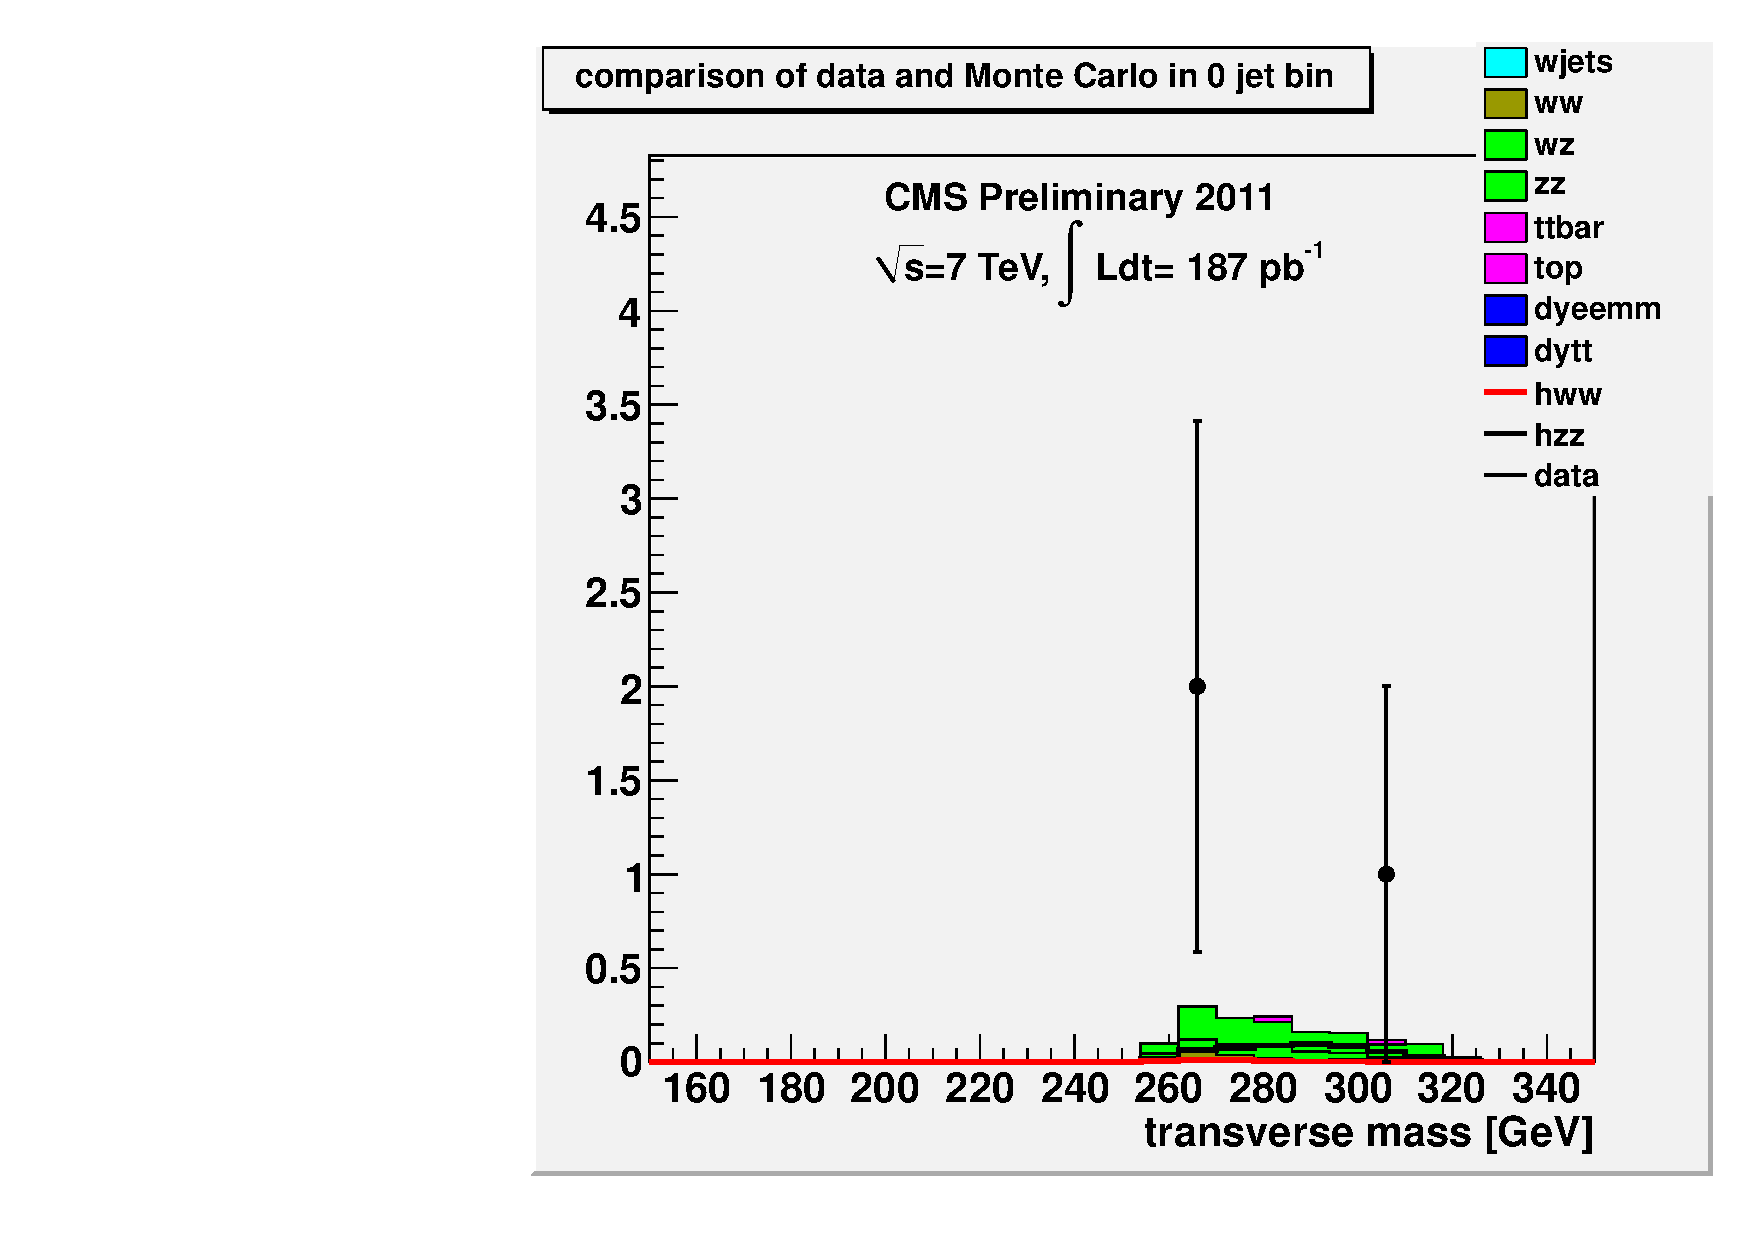
\includegraphics[width=.45\textwidth]{figures/fullselection_0jets_mt.pdf}}
\subfigure[1-Jet]{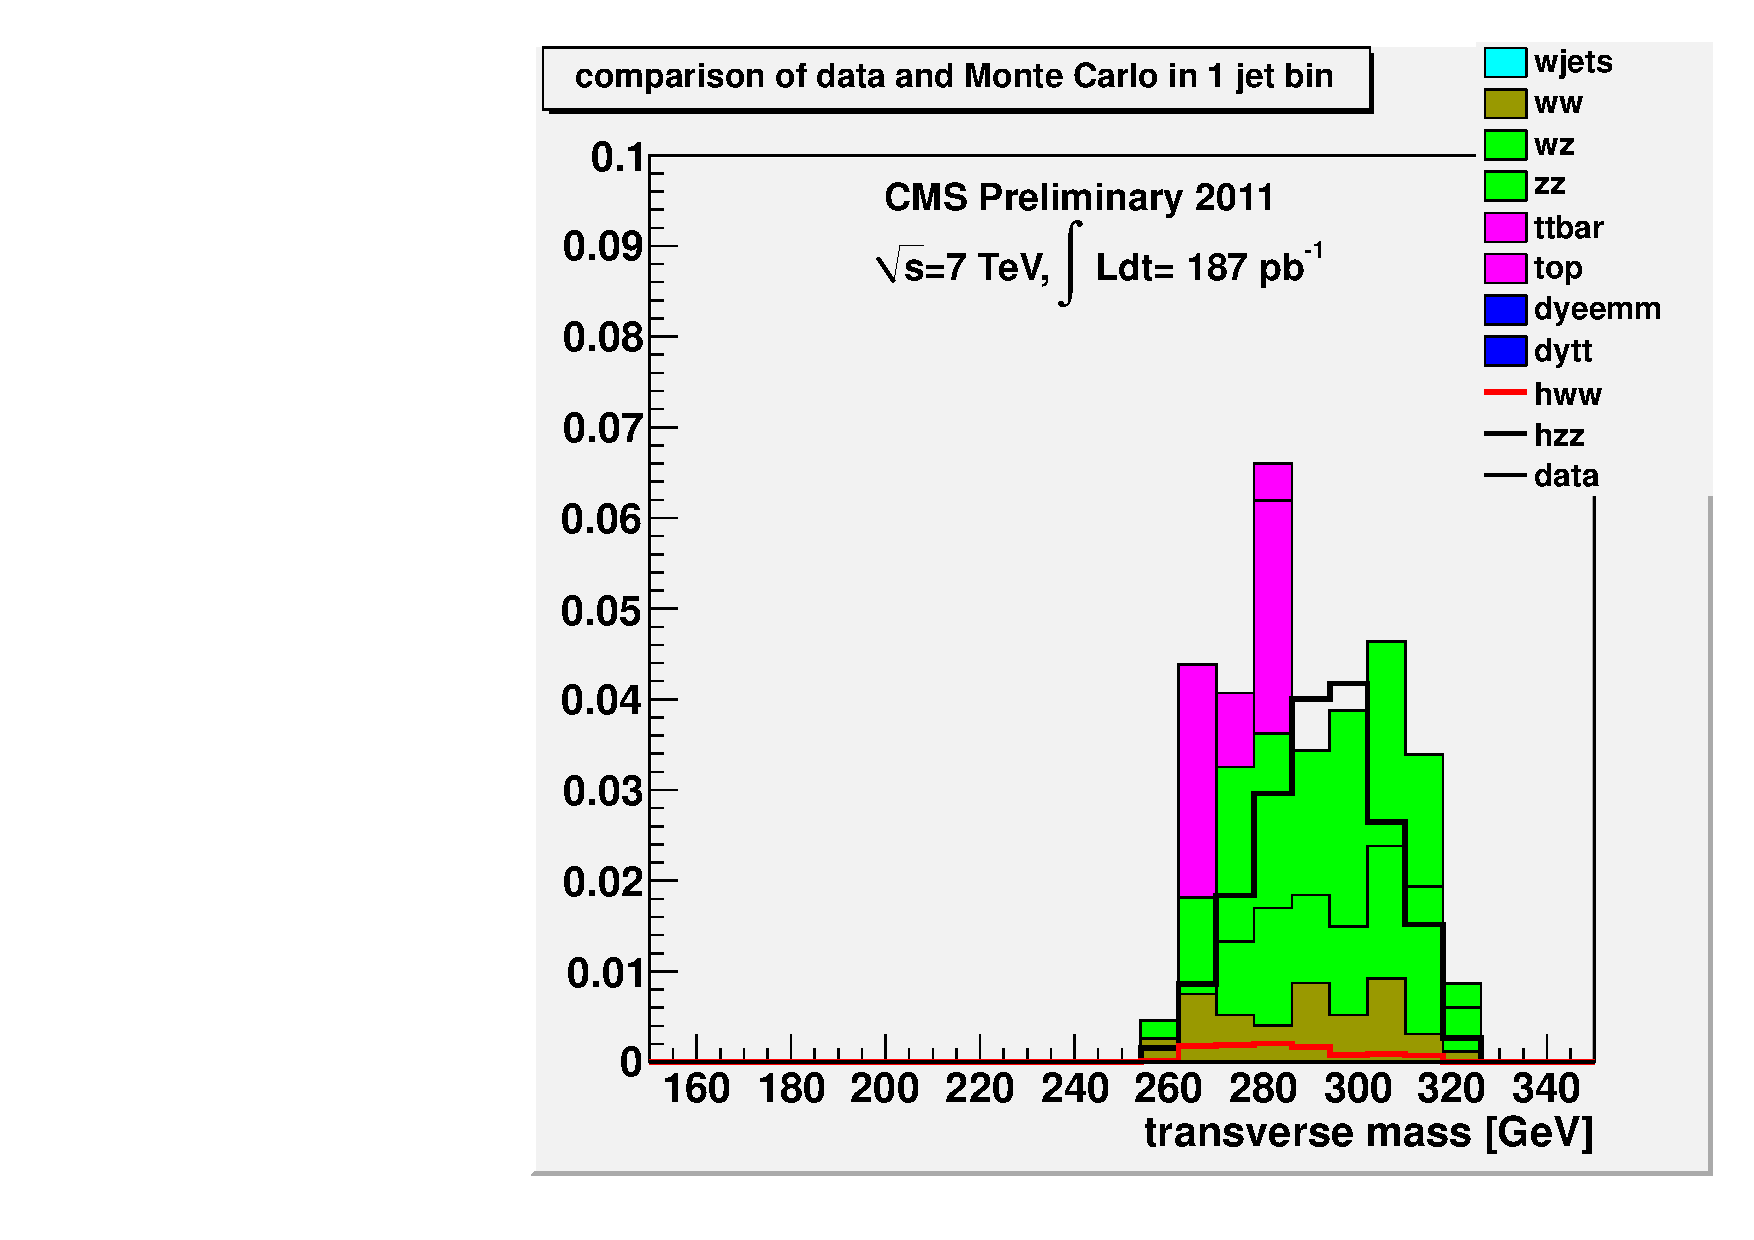
\includegraphics[width=.45\textwidth]{figures/fullselection_1jet_mt.pdf}}
\subfigure[$\geq$2 Jets]{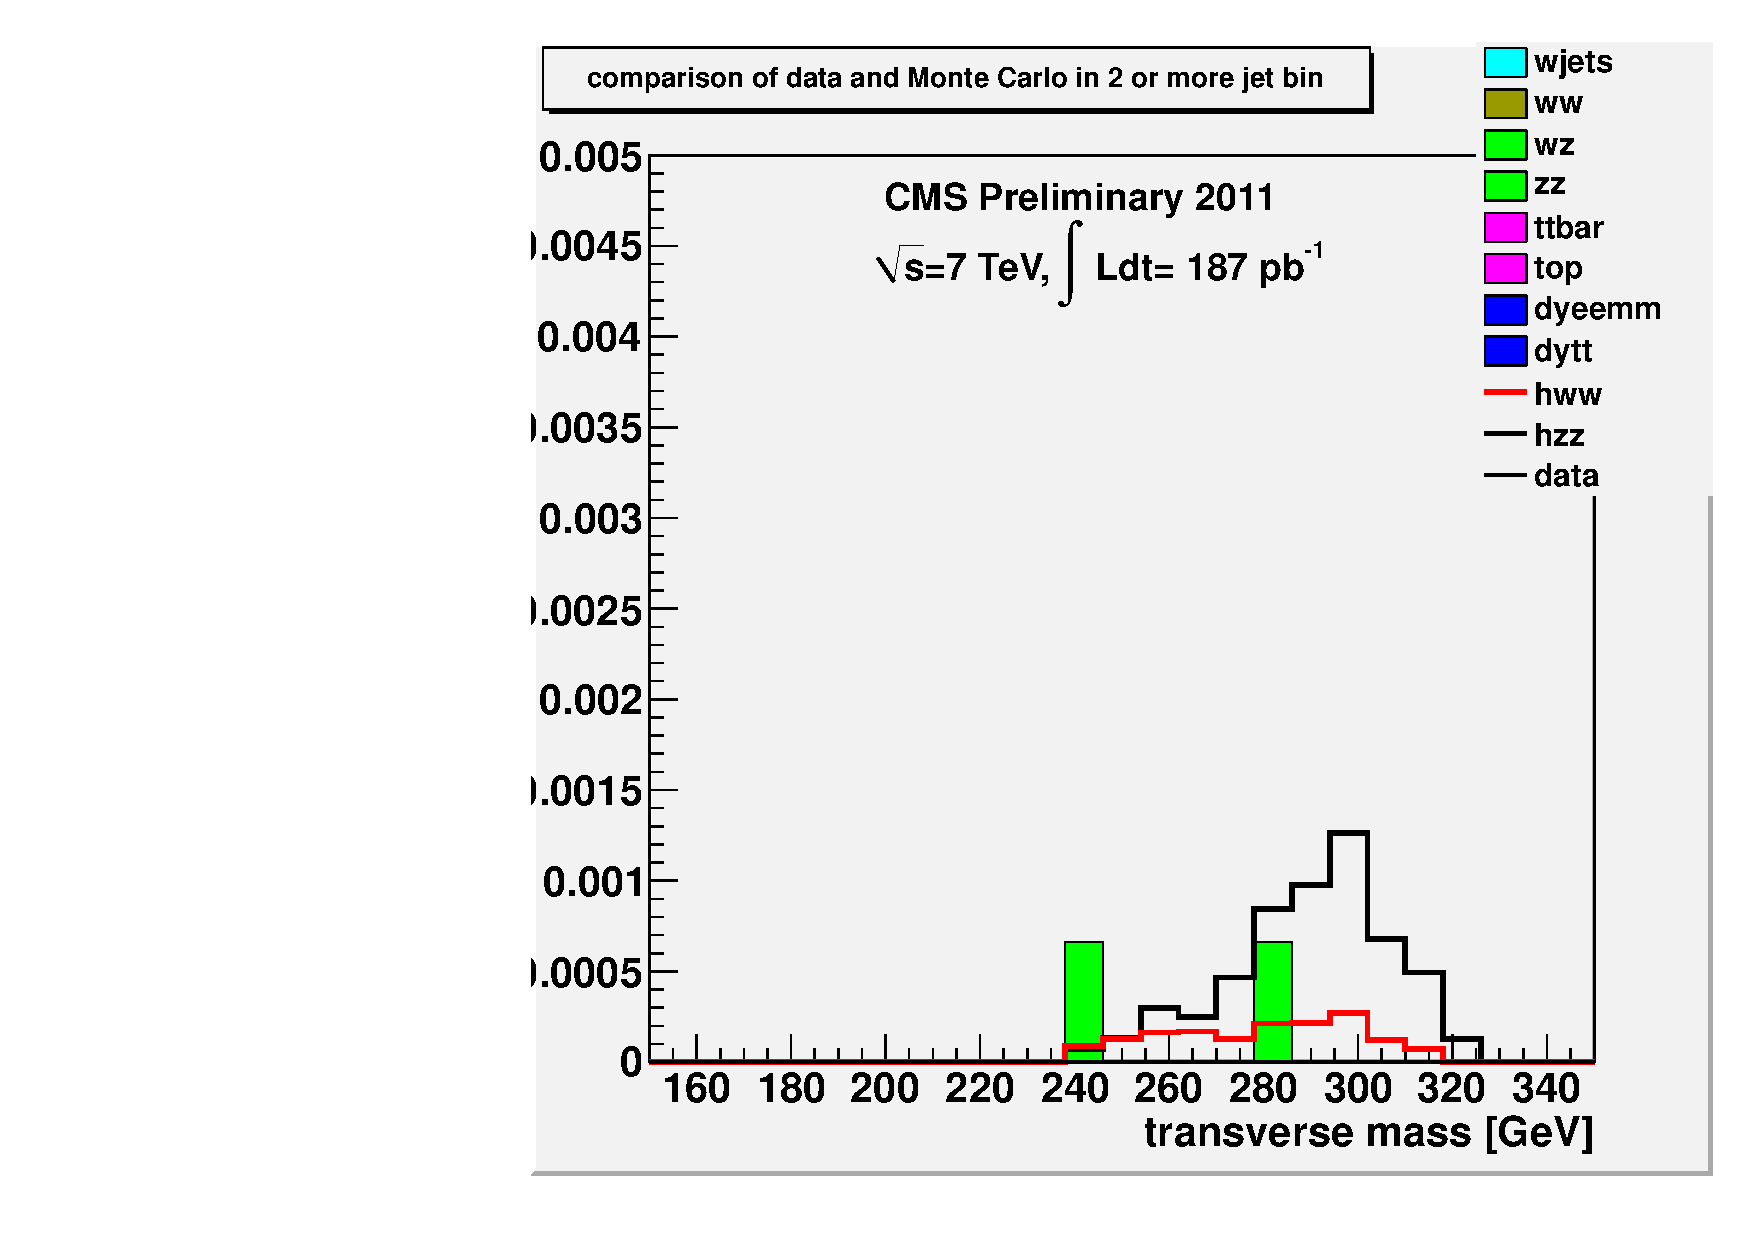
\includegraphics[width=.45\textwidth]{figures/fullselection_2jets_mt.pdf}}
\caption{The above figures display the background, higgs, and data yields as a function of the transverse mass after full 300 GeV selection. No efficiency scale factors were used, but pt reweighting was applied to the higgs MC.}
\end{center}
\end{figure}
%%%%%%%%

%%%%%%%%
\begin{figure}[!hbtp]
\begin{center}
\label{}
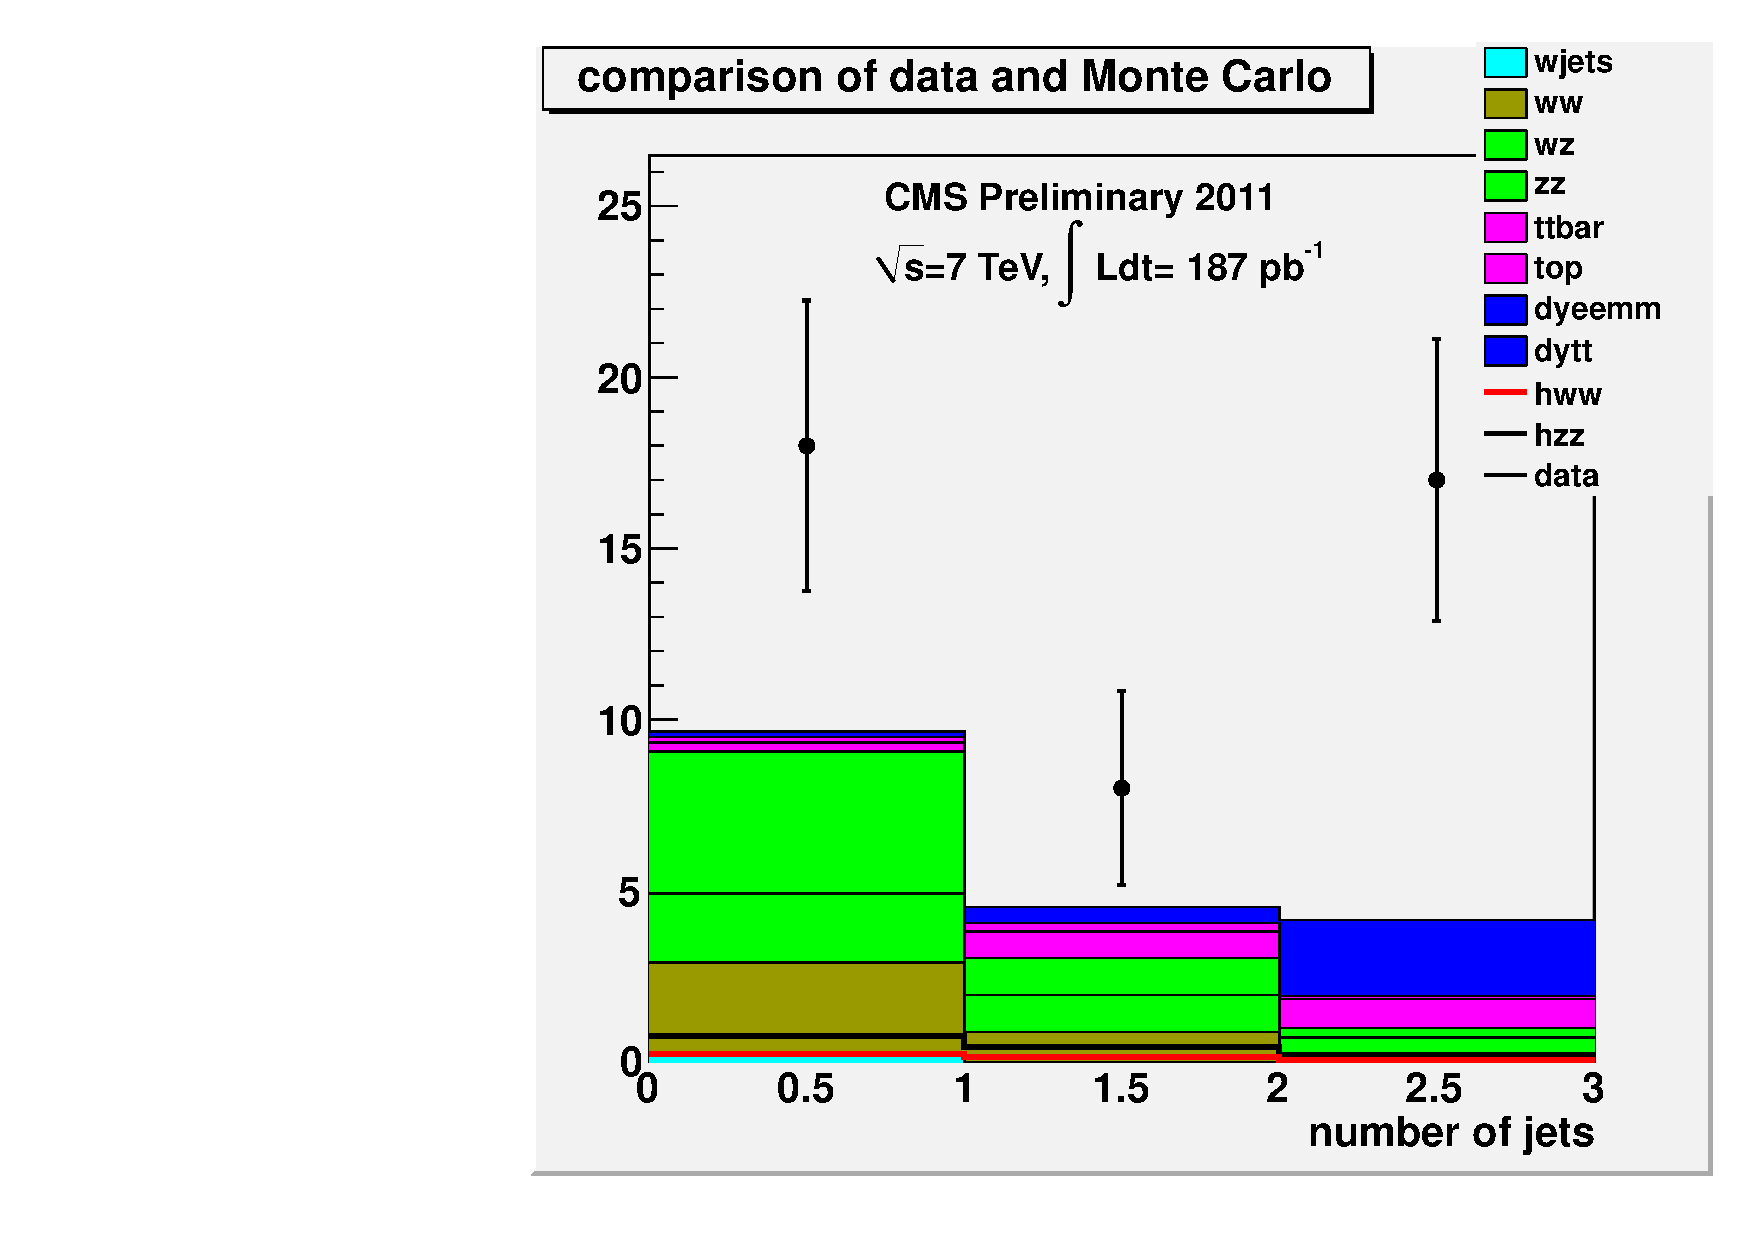
\includegraphics[width=.45\textwidth]{figures/preselection_njets.pdf}
\caption{The above figure displays the background, higgs, and data yields as a function of the number of jets after preselection. No efficiency scale factors were used, but pt reweighting was applied to the higgs MC.}
\end{center}
\end{figure}
%%%%%%%%

%%%%%%%%
\begin{figure}[!hbtp]
\begin{center}
\label{}
\subfigure[0-Jet]{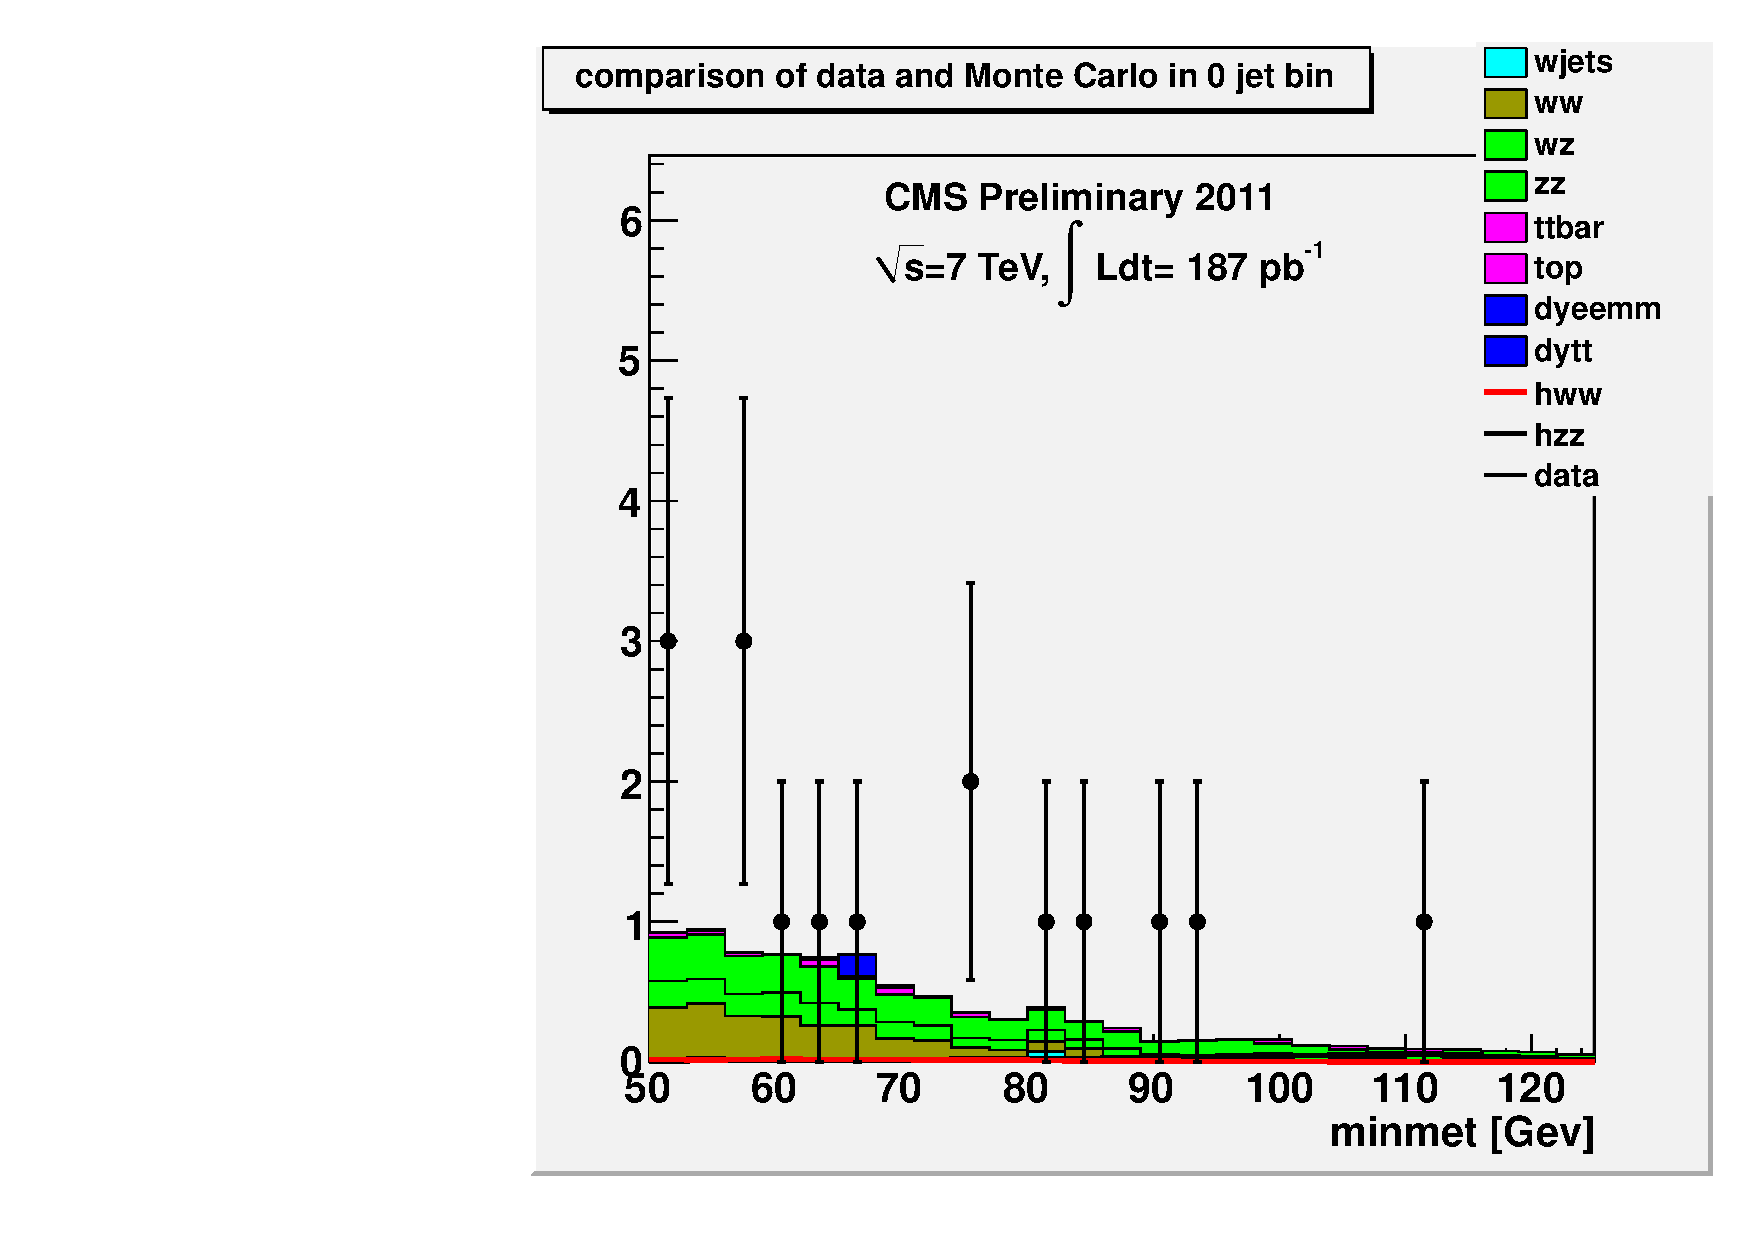
\includegraphics[width=.45\textwidth]{figures/preselection_0jets_minmet.pdf}}
\subfigure[1-Jet]{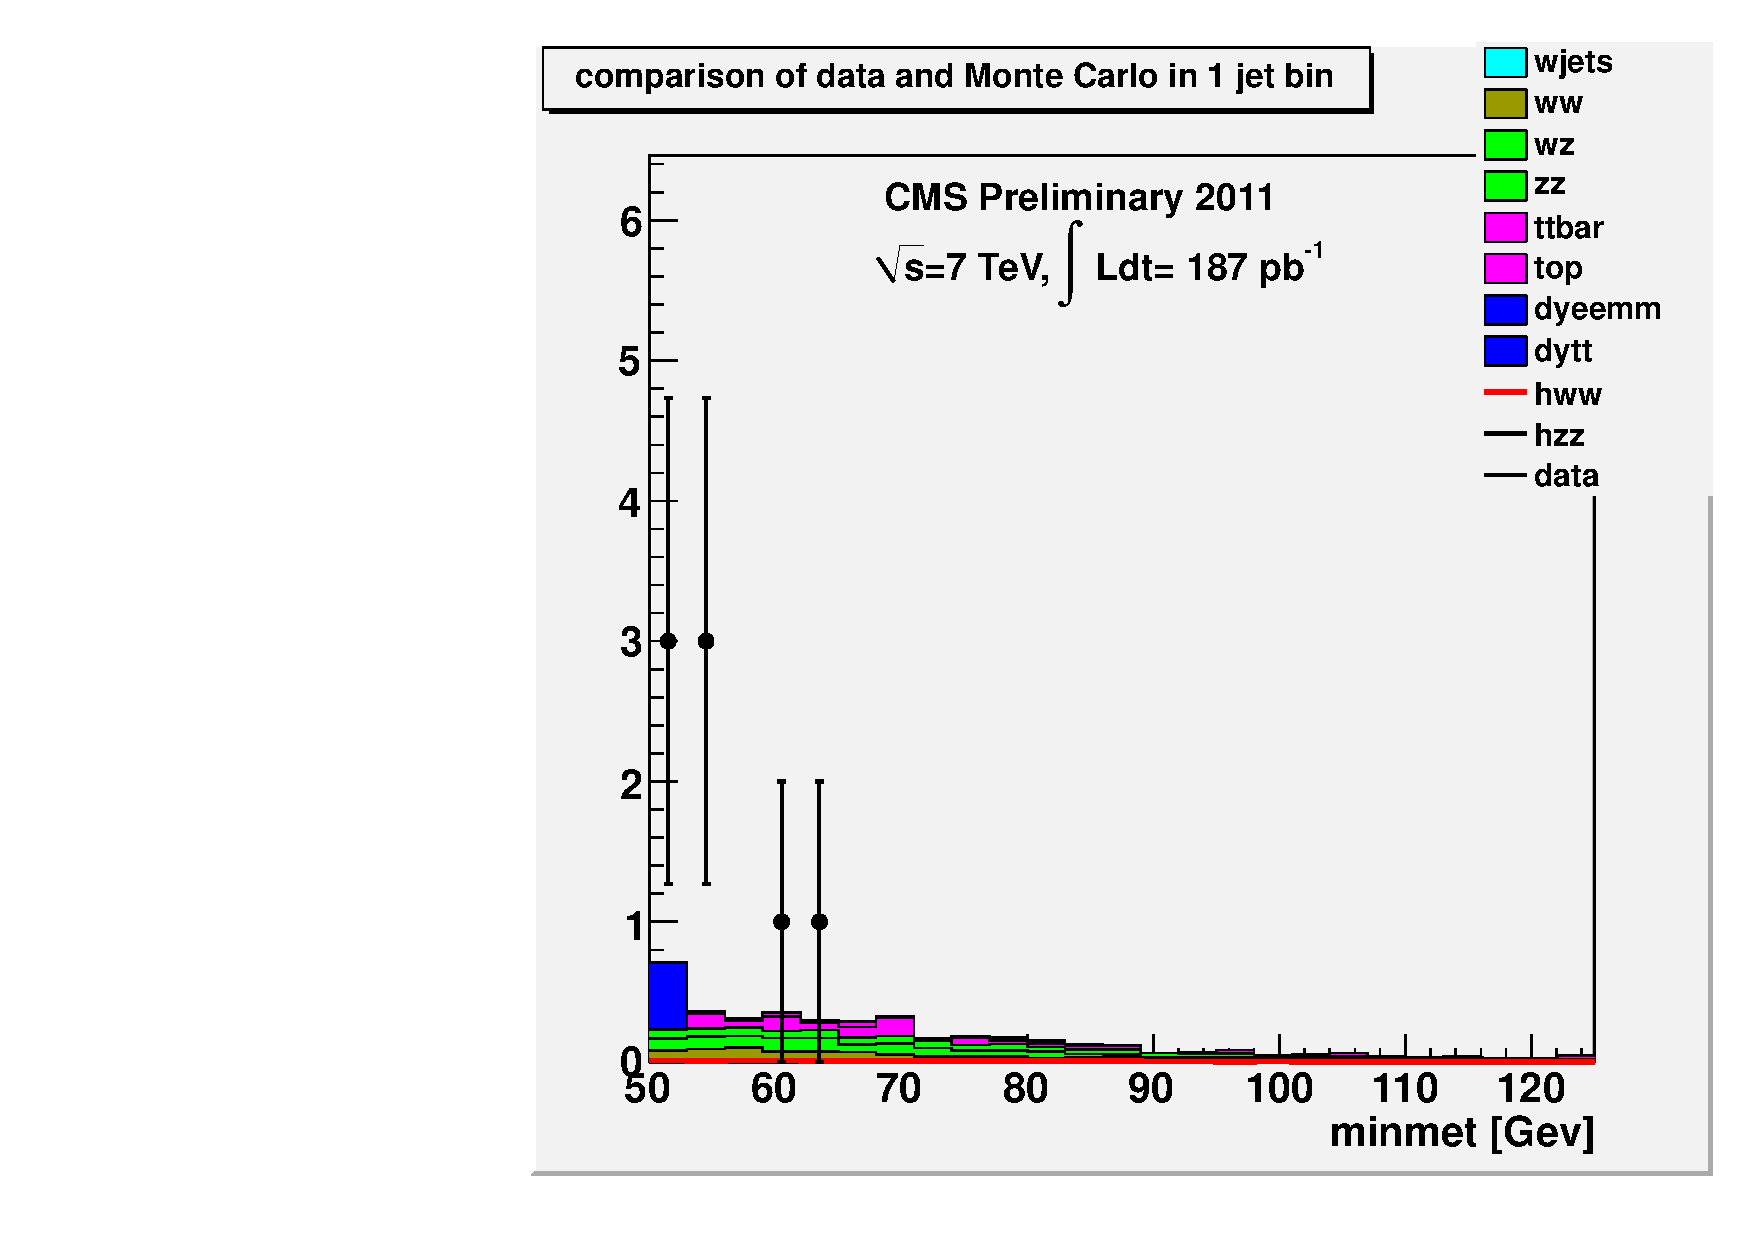
\includegraphics[width=.45\textwidth]{figures/preselection_1jet_minmet.pdf}}
\subfigure[$\geq$2 Jets]{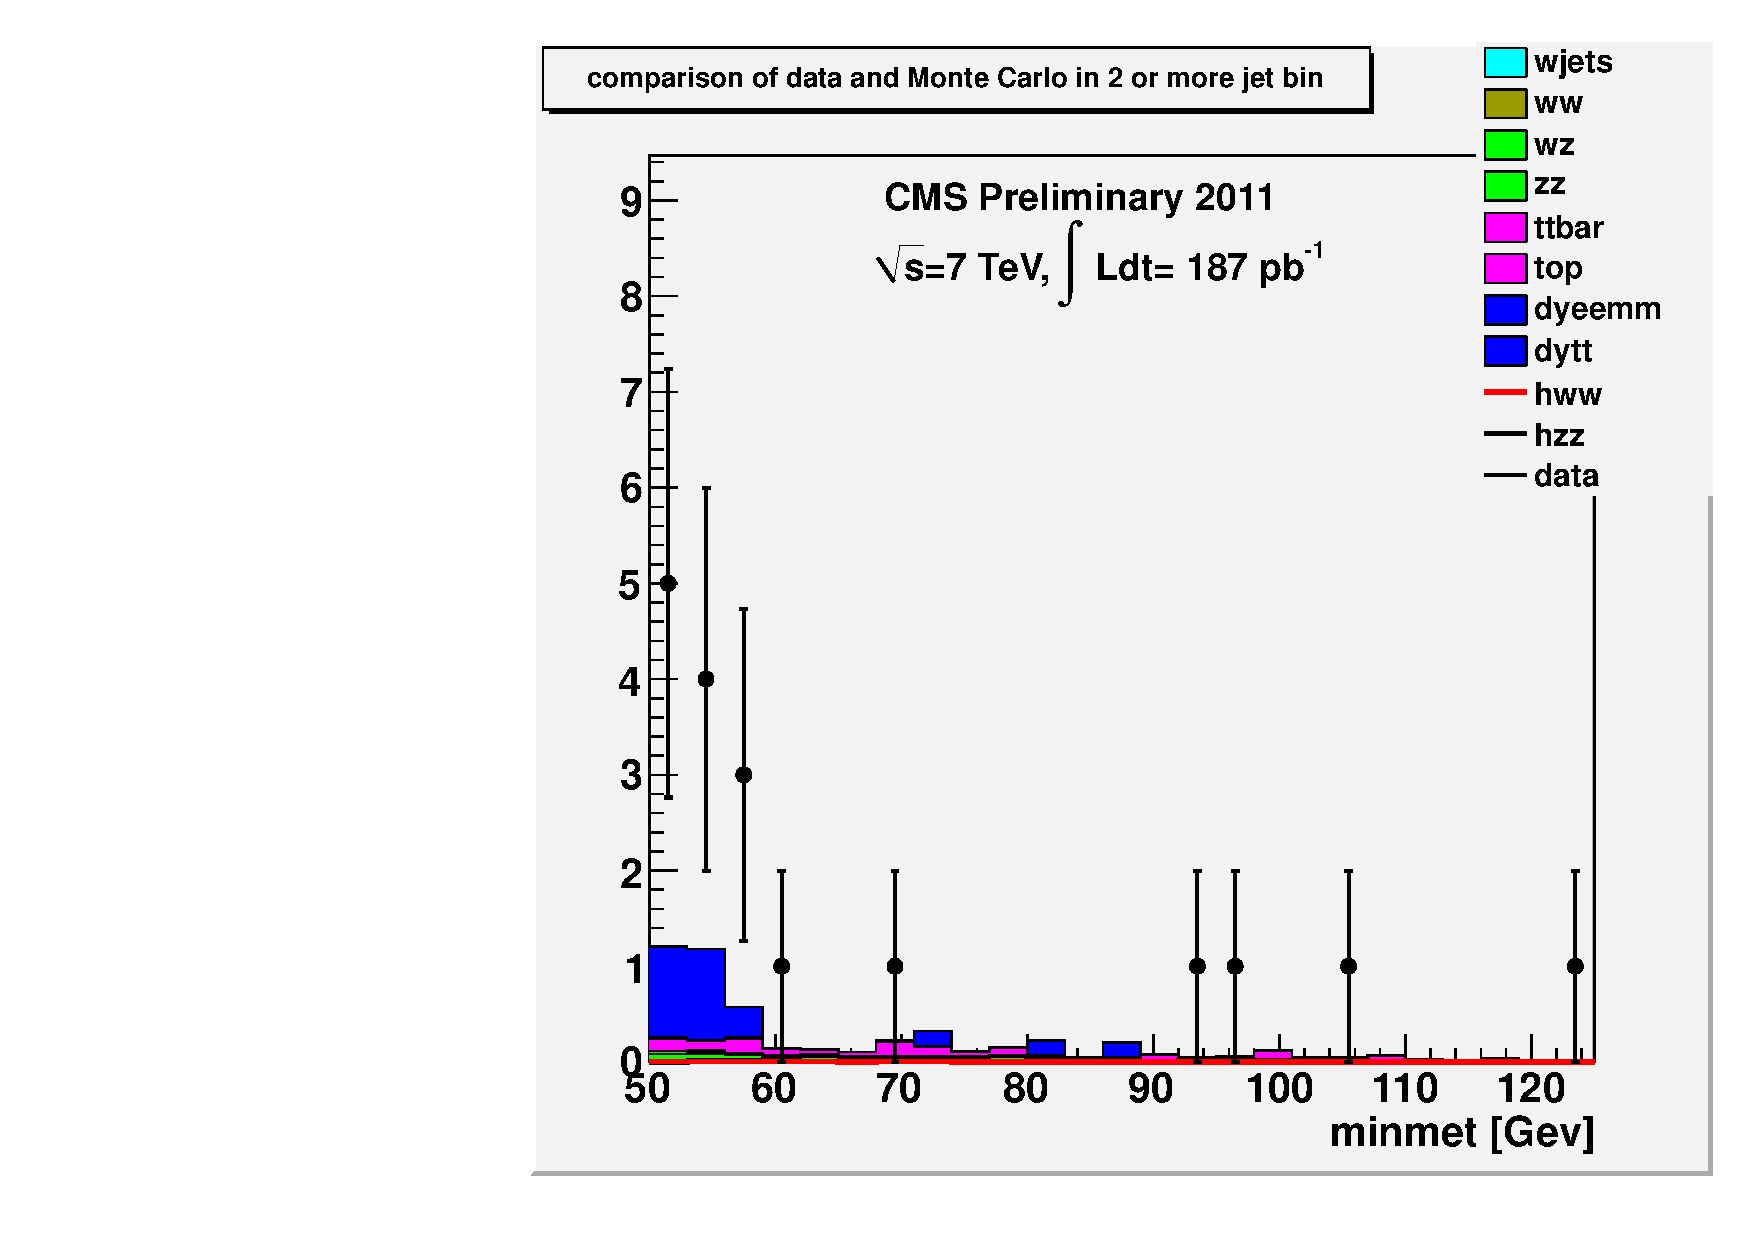
\includegraphics[width=.45\textwidth]{figures/preselection_2jets_minmet.pdf}}
\caption{The above figures display the background, higgs, and data yields as a function of min(met,tracker met) after preselection. No efficiency scale factors were used, but pt reweighting was applied to the higgs MC.}
\end{center}
\end{figure}
%%%%%%%%

%%%%%%%%
\begin{figure}[!hbtp]
\begin{center}
\label{}
\subfigure[0-Jet]{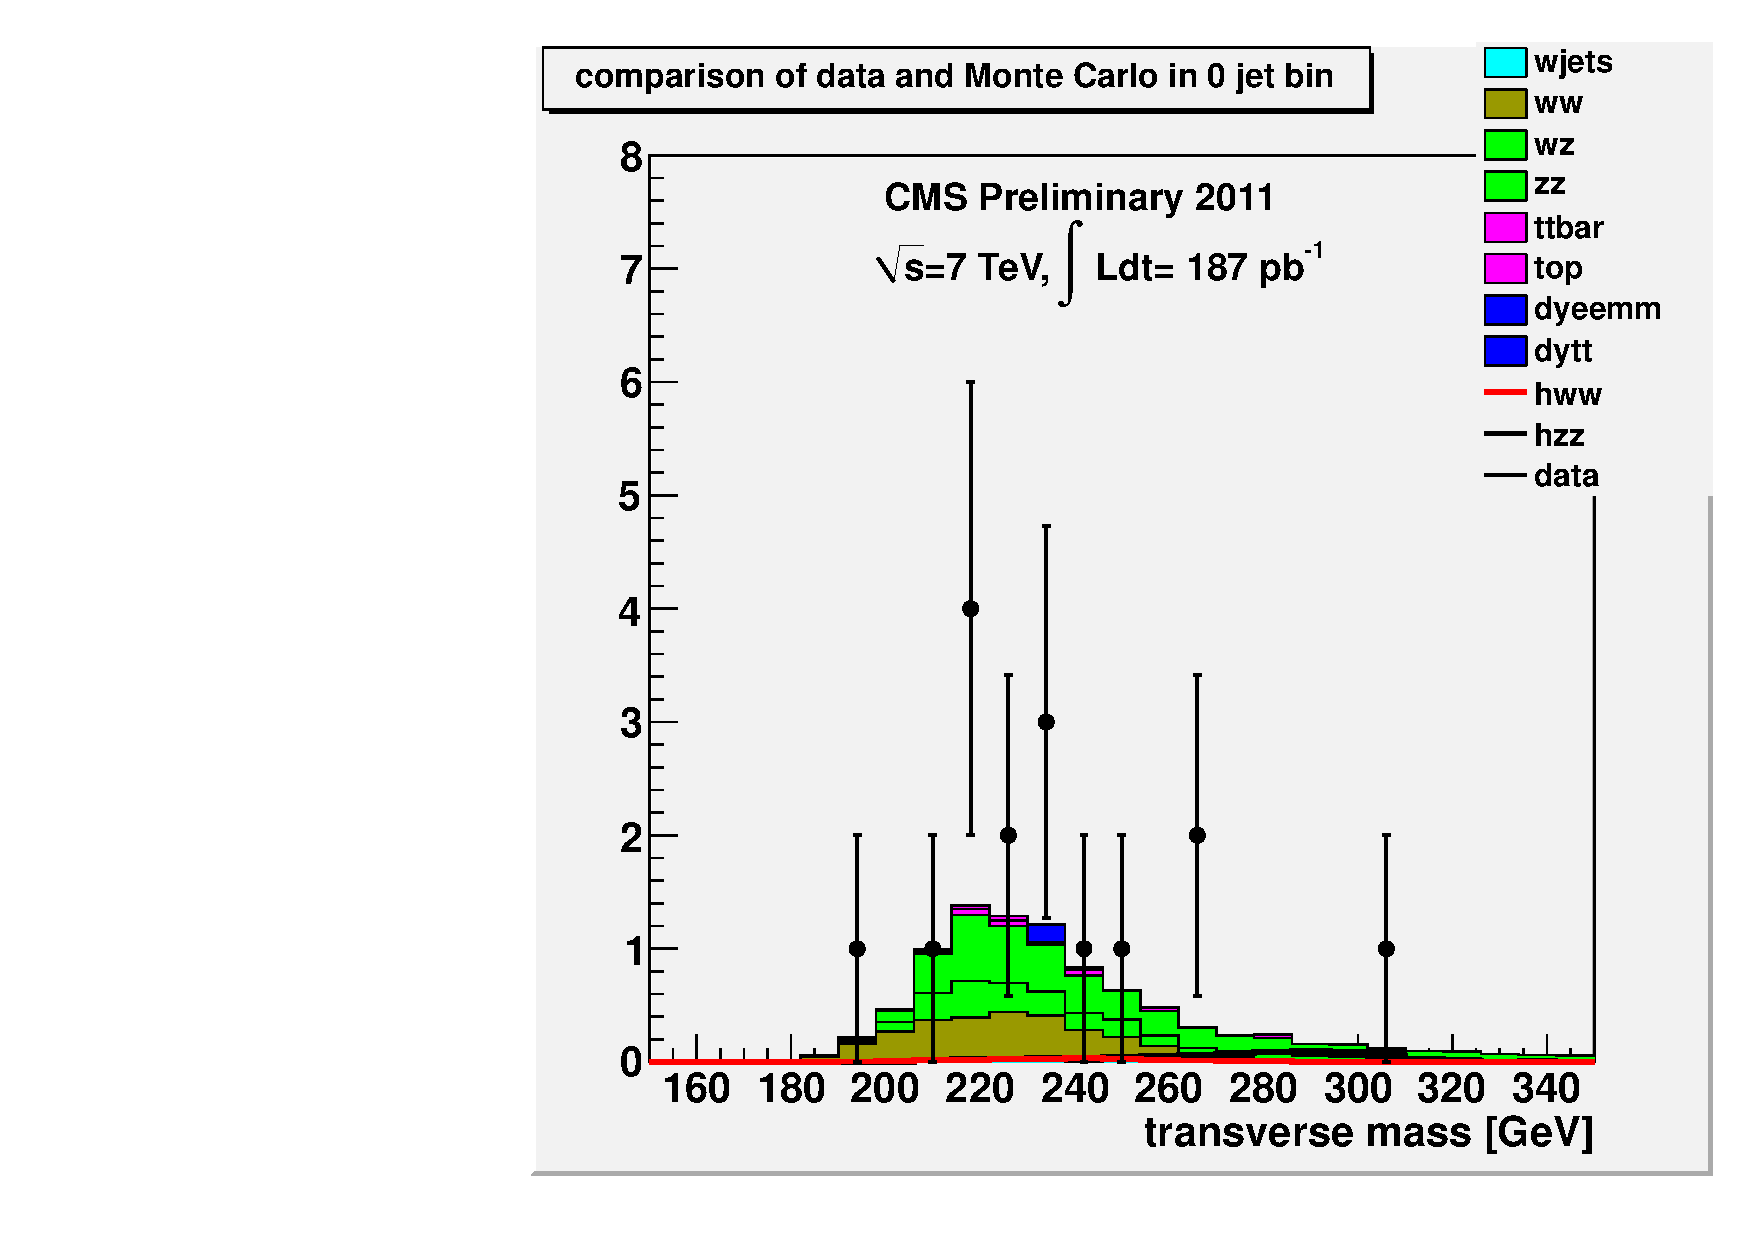
\includegraphics[width=.45\textwidth]{figures/preselection_0jets_mt.pdf}}
\subfigure[1-Jet]{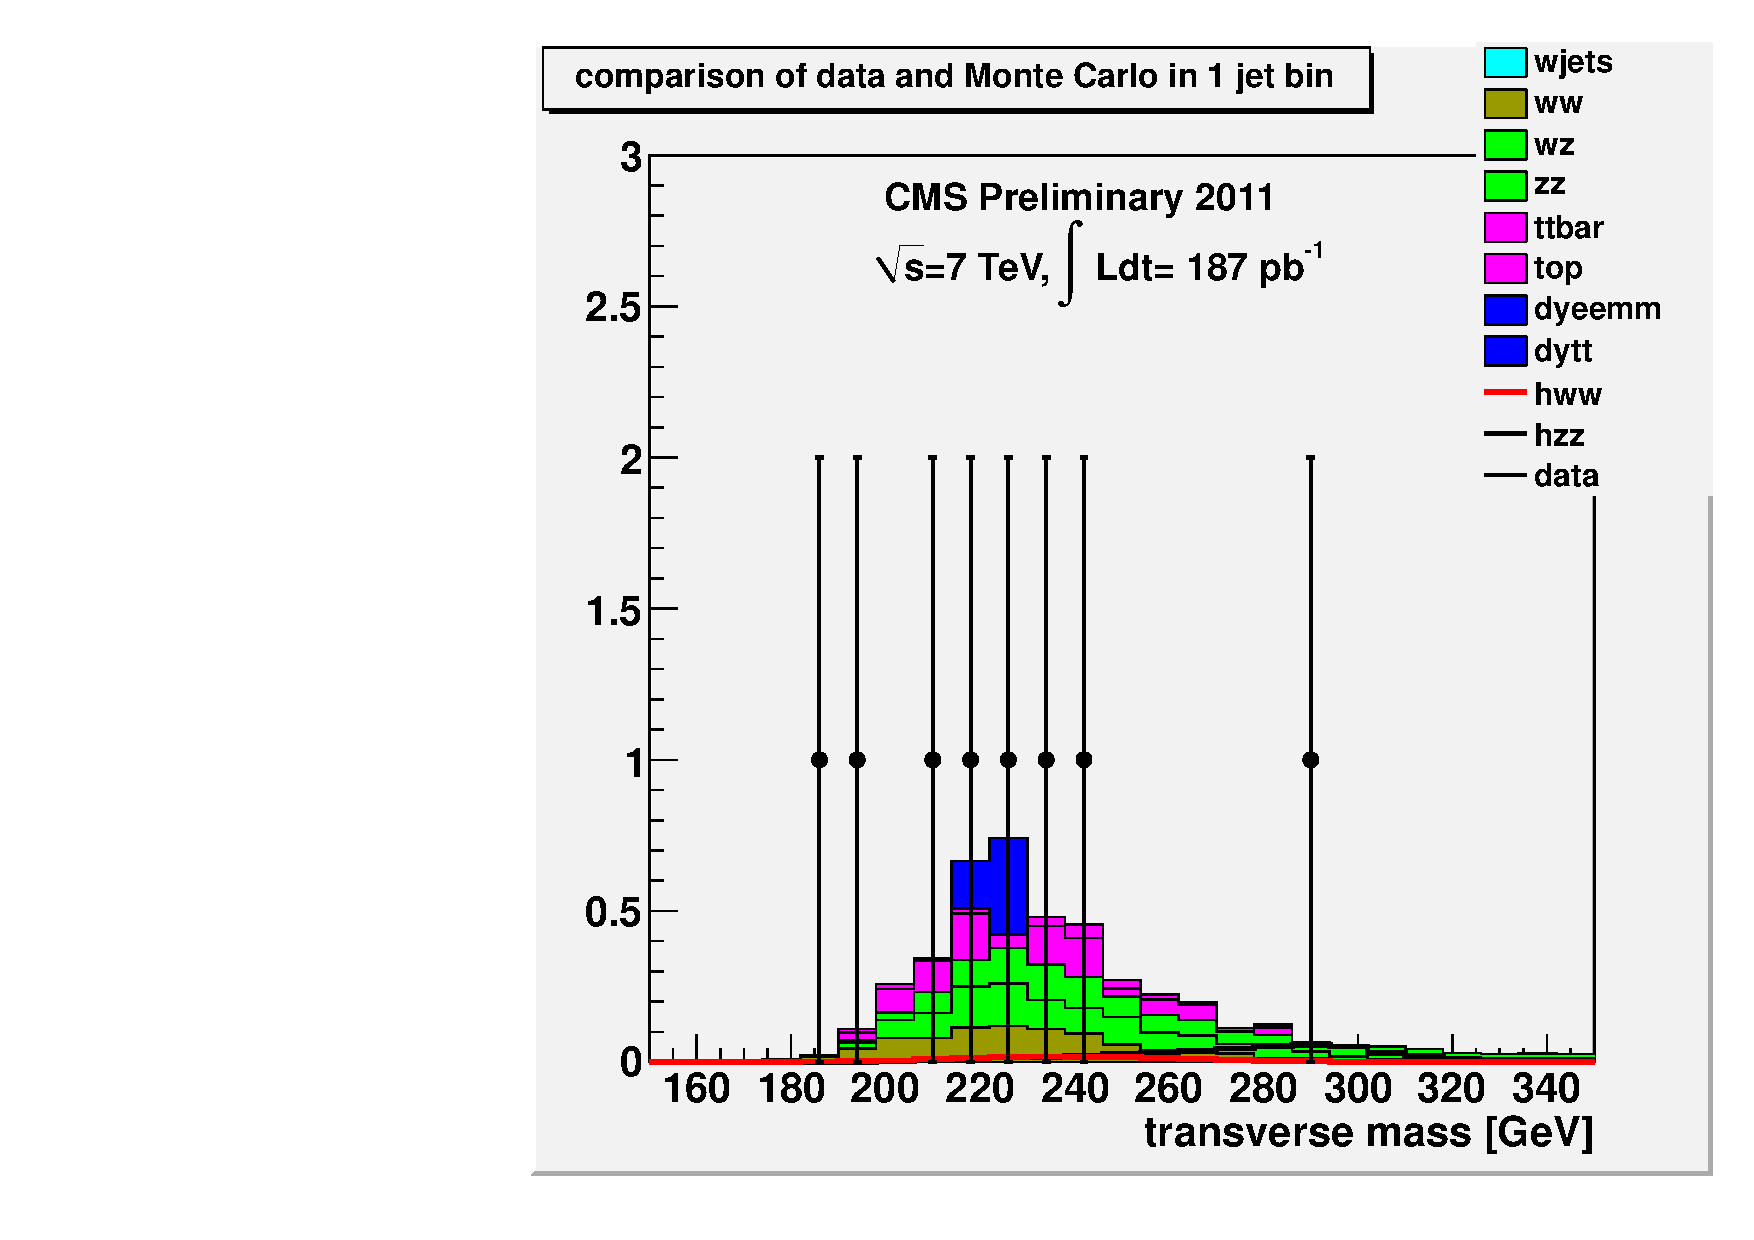
\includegraphics[width=.45\textwidth]{figures/preselection_1jet_mt.pdf}}
\subfigure[$\geq$2 Jets]{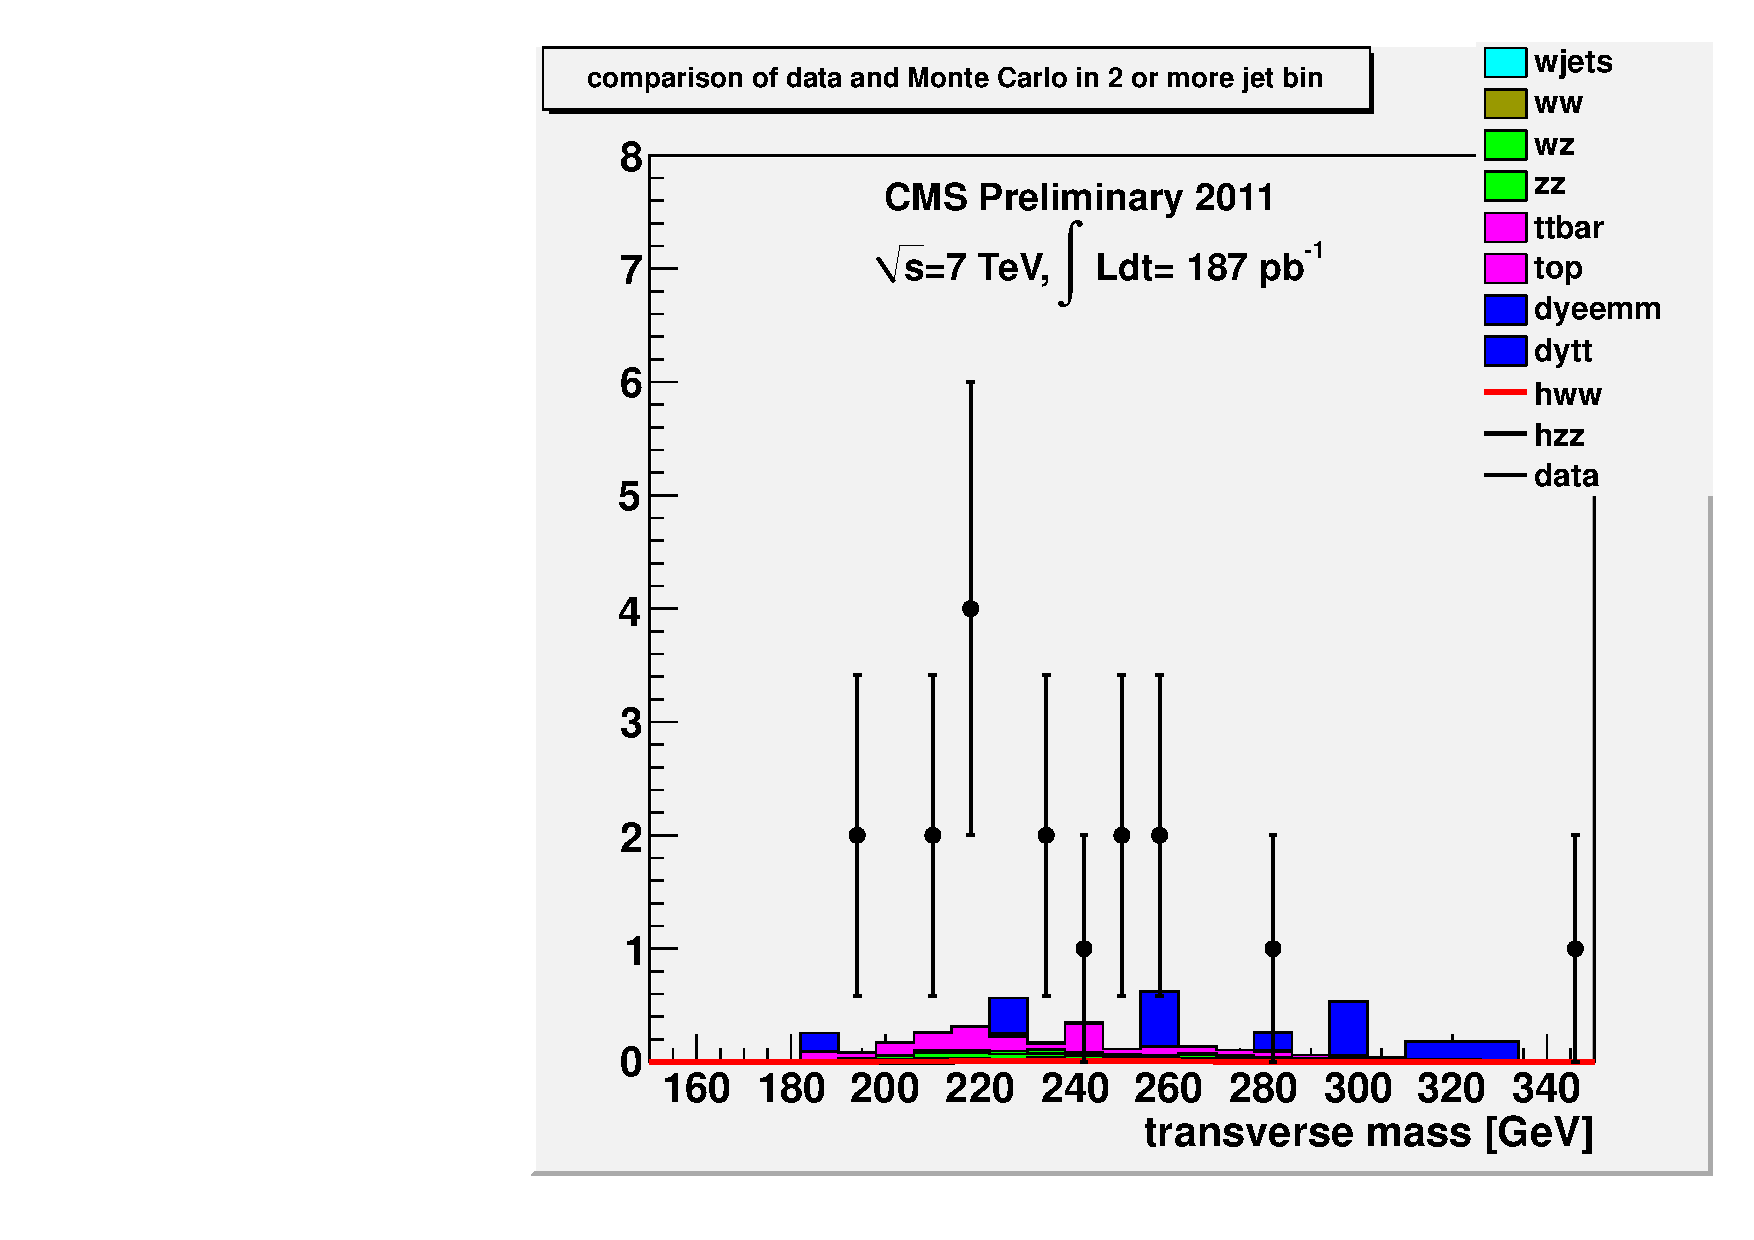
\includegraphics[width=.45\textwidth]{figures/preselection_2jets_mt.pdf}}
\caption{The above figures display the background, higgs, and data yields as a function of the transverse mass after preselection. No efficiency scale factors were used, but pt reweighting was applied to the higgs MC.}
\end{center}
\end{figure}
%%%%%%%%